\documentclass{beamer}

\usepackage[T1]{fontenc}
\usepackage[utf8]{inputenc}
\usepackage[ngerman]{babel}
\usepackage[ngerman]{datetime2}

\usepackage[range-units = single]{siunitx}
\sisetup{detect-weight=true, detect-family=true}

\usepackage{tikz}
\usetikzlibrary{arrows, calc, patterns, intersections, datavisualization}

\DeclareMathOperator{\di}{d\!}					% d
\newcommand{\nint}[2]{\int\limits_{#1}^{#2}\!}	% nice Integral
\newcommand{\prac}[2]{\frac{\partial#1}{\partial#2}} % \frac mit \partial
\newcommand{\drac}[2]{\frac{\di#1}{\di#2}} % \frac mit \di


\mode<presentation>


\title{Gravitationslinseneffekt}
\subtitle{Lichtablenkung an einem Galaxiencluster}
\author{Pascal Stump}
\date{\DTMdate{2017-05-29}}
\institute{HSR Mathematisches Seminar 2017}

\begin{document}

\begin{frame}
  \titlepage
\end{frame}

\begin{frame}
  \frametitle{Ablauf}
  \tableofcontents
\end{frame}


\section{Einleitung}

\begin{frame}
  \frametitle{LRG 3-757}
  \begin{figure}
    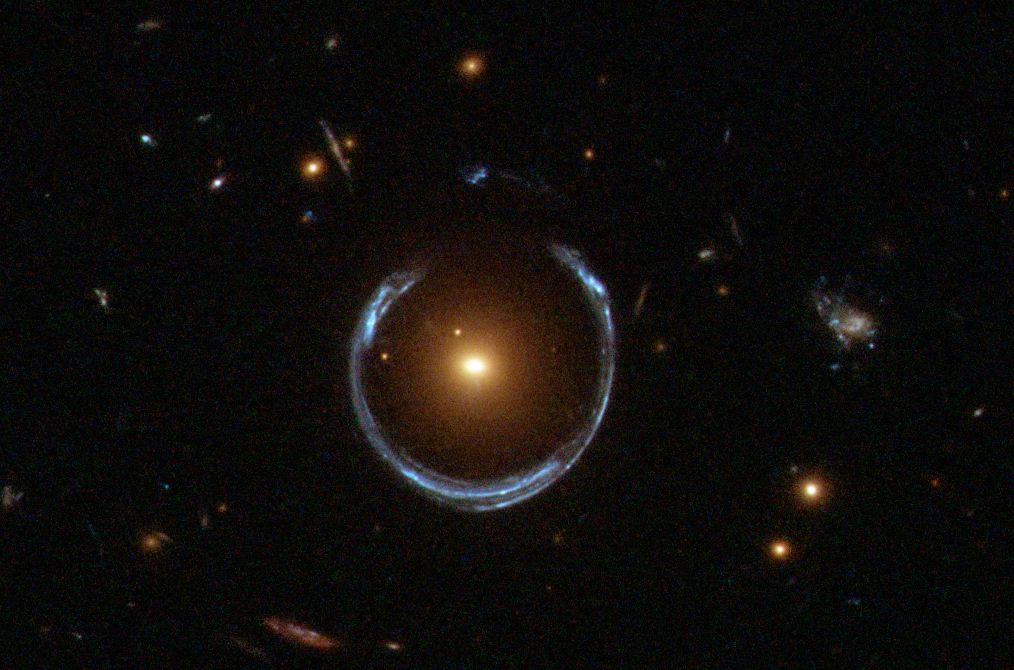
\includegraphics[width=\textwidth]{../images/LRG_3-757}
  \end{figure}
\end{frame}

\begin{frame}
  \frametitle{Einsteinkreuz}
  \begin{figure}
    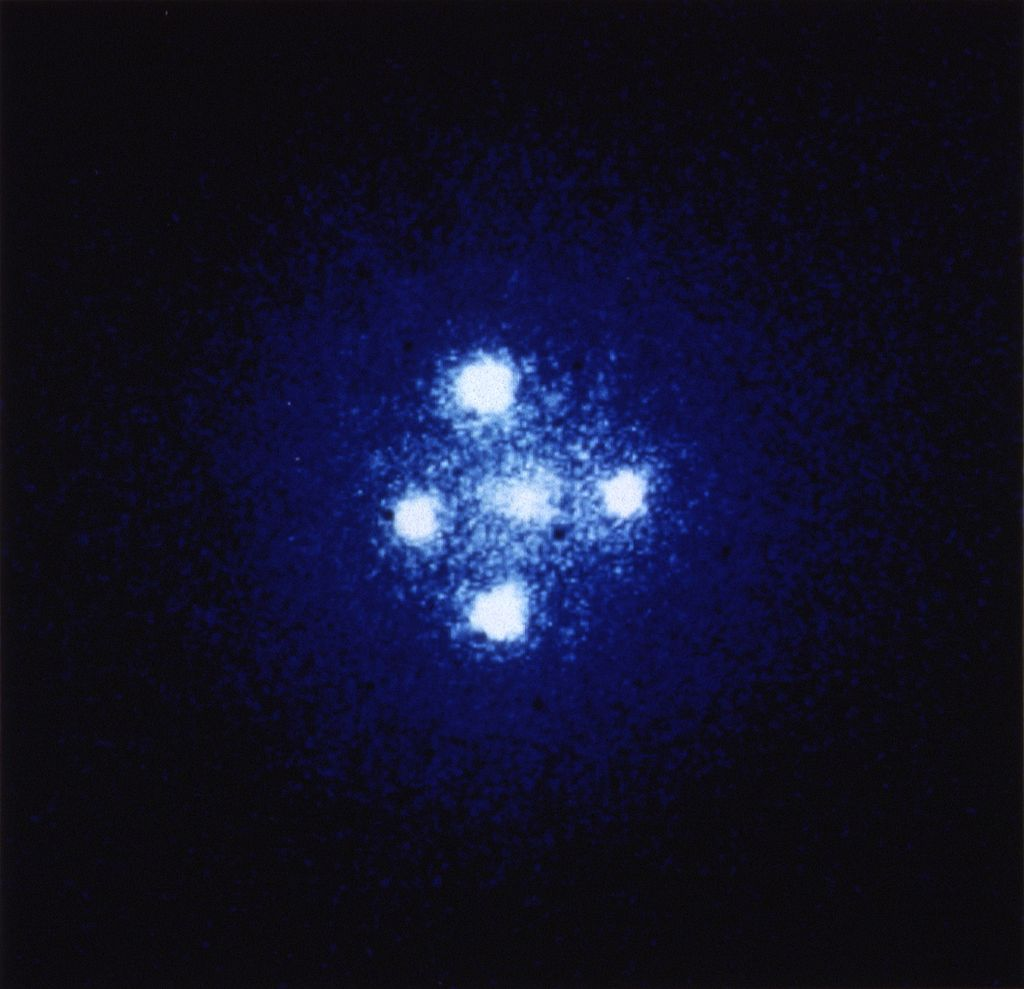
\includegraphics[width=.7\textwidth]{../images/Einstein_cross}
  \end{figure}
\end{frame}

\begin{frame}
  \frametitle{Galaxiencluster Abell 2218}
  \begin{figure}
    \includegraphics[width=\textwidth]{../images/HSTCI_PR00-08}
  \end{figure}
\end{frame}


\section{Linse}
\subsection{``Normale'' Linse}
\begin{frame}
  \frametitle{Prinzip von Huygens}
  \centering
  \begin{tikzpicture}  
    % Delta t
    \only<1>{\foreach \y in {-1}}
    \only<2-3>{\foreach \y in {-1,0}}
    \only<4>{\foreach \y in {-1,0,1}}
      \draw [very thick, color=red] (0,\y) -- (6,\y);

    \only<3->{
      \foreach \x in {1,2,3,4,5}
      \draw [black, fill=white] (\x,0) circle (.6mm);}

    \only<3->{
    \foreach \x in {1,2,3,4,5}
      \draw [blue] (\x,0) ++ (0,1) arc (90:160:1cm)
                   (\x,0) ++ (0,1) arc (90:20:1cm);}

    \draw [very thick, color=red, ->, >=stealth] (-.5,-.5) -- (-.5,0.5);
    \draw [very thick, color=red, ->, >=stealth] (6.5,-.5) -- (6.5,0.5);
  \end{tikzpicture}
\end{frame}


\begin{frame}
  \frametitle{Brechung}
  
  \begin{itemize}
  \item Brechung an Materialübergang
    \begin{equation*}
      \frac{\sin \varepsilon_1}{\sin \varepsilon_2} = \frac{n_2}{n_1}
    \end{equation*}
  \item Brechungsindex
    \begin{equation*}
      n = \frac{c}{u}
    \end{equation*}
  \end{itemize}
\end{frame}

\begin{frame}
  \frametitle{Brechung mit Huygens}
  \centering
  \begin{tikzpicture}
    [every label/.style={color=black}]
  
    % Oberfläche
    \fill [fill=blue!15!white] (0,0) rectangle (6,-2);
    \draw [thick] (0,0) -- (6,0);

    % A und D
    \coordinate[label=below left:$A$] (A) at (3,0);
    \path (A) ++ (2,0) coordinate[label=below right:$D$] (D);

    \draw [very thick, color=red, -<, >=stealth] (A) --++ (150:2.5) node(ray1Start){};
    \path [name path=rayStart] (ray1Start.center) --++ (60:2.5);
    \path [name path=ray2] (A) ++ (2,0) --++ (150:6);
    \draw [very thick, color=red, name intersections={of=rayStart and ray2,
      by=ray2Start}, -<, >=stealth] (A) ++ (2,0) -- (ray2Start);

    \path (ray2Start) ++ (-30:2.5) coordinate[label=above:$B$] (B);
    \draw [color=red] (A) -- (B);

    \only<1>{
      \path
        let \p1 = ($(B)-(D)$)
        in (B) ++ (-30:{veclen(\x1,\y1)}) arc (-30:140:{veclen(\x1,\y1)})
           (B) ++ (150:{veclen(\x1,\y1)}) coordinate (Bs)
           (A) ++ (150:{veclen(\x1,\y1)}) coordinate (As);}
    \only<2->{
      \draw [thick, color=blue] (A) ++ (.8,0) arc (0:-180:.8cm);
      \draw [thick, color=blue]
        let \p1 = ($(B)-(D)$)
        in (B) ++ (-30:{veclen(\x1,\y1)}) arc (-30:140:{veclen(\x1,\y1)})
           (B) ++ (150:{veclen(\x1,\y1)}) coordinate (Bs)
           (A) ++ (150:{veclen(\x1,\y1)}) coordinate (As);}

    \draw [color=red] (As) -- (Bs);

    \only<2->{
    \node [circle] (circleSmall) at (A) [minimum size=2*.8cm,
      inner sep=0]{};}
    \only<3->{
    \draw [color=red] (D) -- (tangent cs:node=circleSmall, point={(D)},
      solution=2) coordinate[label=below left:$C$] (C);}

    \only<4>{
    \path (C) ++ ($ (C)-(A) $) coordinate (Cs);
    \path (D) ++ ($ (C)-(A) $) coordinate (Ds);
    \draw [very thick, color=red, ->, >=stealth] (A) -- (C) -- ($ (C)!1.4!(Cs) $);
    \draw [very thick, color=red, ->, >=stealth] (D) -- ($ (D)!1.4!(Ds) $);
    \draw [color=red] (Cs) -- (Ds);}

    \only<1-2>{\foreach \point in {A,B,D}}
    \only<3->{\foreach \point in {A,B,C,D}}
      \draw [black, fill=white] (\point) circle (.6mm);
  \end{tikzpicture}
\end{frame}

\begin{frame}
  \frametitle{Inhomogenes Material mit Huygens}
  \centering
  \begin{tikzpicture}
    [every label/.style={color=black}]

    \shade [inner color=blue!50!white, outer color=white] (-.6,0.55) circle (1.5cm);

    \coordinate (A) at (0,0);
    \coordinate (B) at (3,0);
    \draw [very thick, color=red] (A) -- (B);

    \path (B) ++ (97:1cm) coordinate (Bs);
    \path (Bs) ++ ($ (A)!1!187:(B) $) coordinate (As);
    \draw [very thick, color=red] (As) -- (Bs);

    \path (Bs) ++ (104:1cm) coordinate (Bss);
    \path (Bss) ++ ($ (A)!1!194:(B) $) coordinate (Ass);
    \draw [very thick, color=red] (Ass) -- (Bss);

    \draw [very thick, color=red] (A) ++ (0,-1) --++ ($ (B)-(A) $);
    \draw [very thick, color=red] (Bss) ++ (104:1cm) --++ ($ (A)!1!194:(B) $);
  \end{tikzpicture}
\end{frame}


\subsection{Gravitationslinse}
\begin{frame}
  \frametitle{Gravitationslinse (Punktquelle)}
  \begin{itemize}
  \item schwache Gravitationsfelder
  \item \(\rightarrow\) nur Zeitveränderung
    \begin{align*}
      g_{00} &= 1 +\frac{2\varphi}{c^2} &\varphi &= -\frac{KM}{r}
    \end{align*}
  \end{itemize}
\end{frame}

\begin{frame}
  \frametitle{Zeitveränderung}
  \begin{tikzpicture}[scale = 1.7]
    \datavisualization[scientific axes = clean,
                     y axis = {grid,
                               label=\(\tilde{t}\) von \(1\) bis \(0.05\),
                               min value = 0,
                               max value = 1},
                     x axis = {grid,
                               label=\(r\) in \si{\meter},
                               min value = 0,
                               max value = 60000},
                     visualize as smooth line/.list={ch1},
                     ch1={style=very thick},
                     style sheet=vary hue,
                     %style sheet=vary dashing,
                     %ch1={label in legend={text=Mittenkavität}},
                     ]
                    
    data [set=ch1,headline={x, y}, read from file=../source/bsp1.csv];
  \end{tikzpicture}
\end{frame}

\begin{frame}
  \frametitle{Model einer Gravitationslinse}
  \begin{figure}
    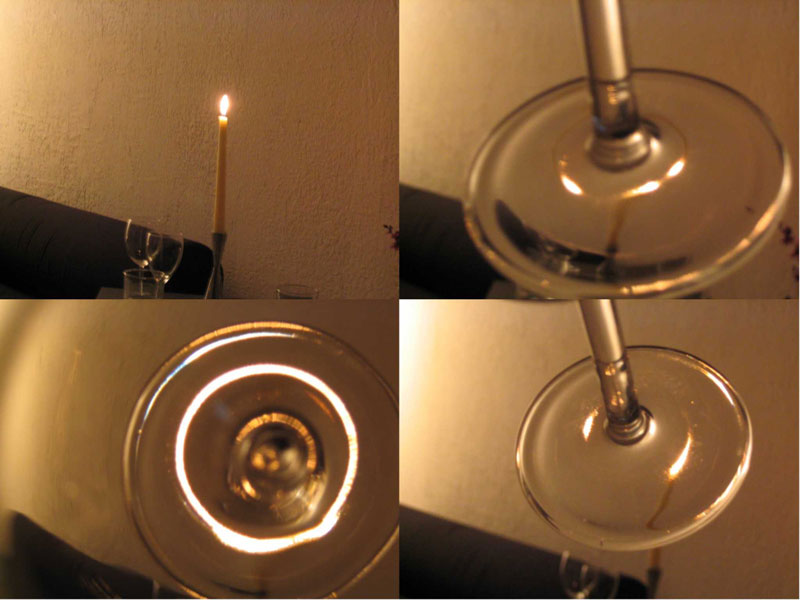
\includegraphics[width=\textwidth]{../images/model_grav_lens}
  \end{figure}
\end{frame}

\section{Euler-Lagrange Gleichung}
\begin{frame}
  \frametitle{Euler-Lagrange}
  \begin{itemize}
  \item kürzeste Laufzeit
    \begin{equation*}
      t = \frac{s}{v}
    \end{equation*}
  \item \(\rightarrow\) Euler-Lagrange
    \begin{equation*}
      I = \nint{t_0}{t_1} F\bigl(x^{\alpha}(t), \dot{x}^{\alpha}(t),t\bigr)\di t
    \end{equation*}
  \end{itemize}
\end{frame}

\begin{frame}
  \frametitle{Zeitintegral (1)}
  \begin{equation*}
    I = \nint{}{}
    \only<2>{\underbrace}
    { \sqrt{\dot{x}(l)^2+\dot{y}(l)^2+\dot{z}(l)^2} }_{\only<2>{s}} \cdot
    \only<3>{\underbrace}
    {  \frac{n\bigl(x(l),y(l),z(l)\bigr)}{c} }_{\only<3>{\dfrac{1}{v}}}
    \di l
  \end{equation*}
\end{frame}

\begin{frame}
  \frametitle{Zeitintegral (2)}
  \begin{equation*}
    I = \frac{1}{c} \nint{}{}
    \sqrt{\dot{x}(l)^2+\dot{y}(l)^2+\dot{z}(l)^2} \cdot
    n\bigl(x(l),y(l),z(l)\bigr)
    \di l
  \end{equation*}
  \vspace{.5cm}
  \only<2->{
    \begin{equation*}
      L = \sqrt{\dot{x}(l)^2+\dot{y}(l)^2+\dot{z}(l)^2} \cdot
      n\bigl(x(l),y(l),z(l)\bigr)
    \end{equation*}}
  \vspace{.5cm}
  \only<3->{
    \begin{equation*}
      F = L^2 = (\dot{x}^2+\dot{y}^2+\dot{z}^2) n^2
    \end{equation*}}
\end{frame}

\begin{frame}
  \frametitle{Euler-Lagrange}
  \begin{equation*}
    0 = \prac{F}{x} - \drac{}{l}\prac{F}{\dot{x}}
  \end{equation*}
  \vspace{.5cm}
  \begin{align*}
    \prac{F}{x} &= (\dot{x}^2+\dot{y}^2+\dot{z}^2) 2n \prac{n}{x}\\
    \prac{F}{\dot{x}} &= 2\dot{x}n^2\\
    \drac{}{l}\prac{F}{\dot{x}} &= 2\ddot{x}n^2 + 4\dot{x}n
                                  \left(\prac{n}{x}\dot{x} +
                                  \prac{n}{y}\dot{y} +
                                  \prac{n}{z}\dot{z} \right)
  \end{align*}
\end{frame}

\begin{frame}
  \frametitle{Logarithmische Differentiation}
  \begin{equation*}
    \ddot{x} = (-\dot{x}^2+\dot{y}^2+\dot{z}^2) \frac{1}{n}\prac{n}{x} -
    2\dot{x}\dot{y} \frac{1}{n}\prac{n}{y} - 2\dot{x}\dot{z} \frac{1}{n}\prac{n}{z}
  \end{equation*}
  \only<2->{
    \vspace{.5cm}
    \begin{equation*}
      \frac{1}{n}\prac{n}{x} = \prac{\ln n}{x}
    \end{equation*}}
  \only<3->{
    \vspace{.5cm}
    \begin{equation*}
      \ddot{x} = (-\dot{x}^2+\dot{y}^2+\dot{z}^2) \prac{\ln n}{x} -
      2\dot{x}\dot{y} \prac{\ln n}{y} - 2\dot{x}\dot{z} \prac{\ln n}{z}
    \end{equation*}}
\end{frame}

\begin{frame}
  \frametitle{Gravitationspotential}
  \begin{equation*}
    \ddot{x} = (-\dot{x}^2+\dot{y}^2+\dot{z}^2) \prac{\ln n}{x} -
    2\dot{x}\dot{y} \prac{\ln n}{y} - 2\dot{x}\dot{z} \prac{\ln n}{z}
  \end{equation*}
  \vspace{.5cm}
  \begin{align*}
    n &\approx 1-\frac{2\varphi}{c^2} &\frac{\varphi}{c^2} &\ll 1
    &\rightarrow \ln n &\approx -\frac{2\varphi}{c^2}
  \end{align*}
  \only<2->{
    \vspace{.5cm}
    \begin{align*}
      \varphi &= -\frac{KM}{r} &r &= \sqrt{(x-x_L)^2+(y-y_L)^2+(z-z_L)^2}
    \end{align*}}
\end{frame}

\begin{frame}
  \frametitle{2D, Punktquelle auf \(x\)-Achse}
  \begin{align*}
    \ddot{x} &= -\frac{2(-\dot{x}^2+\dot{y}^2)(x-x_L)KM}
               {c^2\sqrt{(x-x_L)^2+y^2}^3}+
               \frac{4\dot{x}^2yKM}{c^2\sqrt{(x-x_L)^2+y^2}^3}\\
    \ddot{y} &= +\frac{4\dot{x}\dot{y}(x-x_L)KM}{c^2\sqrt{(x-x_L)^2+y^2}^3}
               - \frac{2(\dot{x}^2-\dot{y}^2)yKM}
               {c^2\sqrt{(x-x_L)^2+y^2}^3}
  \end{align*}
\end{frame}

\begin{frame}
  \frametitle{Substitution}
  \begin{columns}
    \begin{column}{.2\textwidth}
      \begin{align*}
        x(1) &= x\\
        x(2) &= \dot{x}\\
        x(3) &= y\\
        x(4) &= \dot{y}
      \end{align*}
    \end{column}
    \begin{column}{.8\textwidth}
      \only<2>{
      \begin{align*}
        \dot{x}(1) &= x(2)\\
        \dot{x}(2) &= -\frac{2(-x(2)^2+x(4)^2)(x(1)-x_L)KM}
                     {c^2\sqrt{(x(1)-x_L)^2+x(3)^2}^3} + \ldots\\
        \dot{x}(3) &= x(4)\\
        \dot{x}(4) &= +\frac{4x(2)x(4)(x(1)-x_L)KM}
                     {c^2\sqrt{(x(1)-x_L)^2+x(3)^2}^3} - \ldots
      \end{align*}}
    \end{column}
  \end{columns}
\end{frame}


\section{Lichtablenkung an der Sonne}
\begin{frame}
  \frametitle{Lichtablenkung an der Sonne}
  \begin{itemize}
  \item Werte
    \begin{align*}
      x_L &\approx \SI{150e6}{\kilo\meter} &M &\approx
                                                \SI{2e30}{\kilogram}
      &R &\approx \SI{700e3}{\kilo\meter}
    \end{align*}
  \item Winkeländerung \(\approx \SI{1.77}{''}\)\quad (\(\SI{1.75}{''}\))
  \end{itemize}
\end{frame}

\begin{frame}
  \frametitle{Lichtablenkung an der Sonne}
  \begin{tikzpicture}[scale = 1.7]
    \datavisualization[scientific axes = clean,
                     y axis = {grid,
                               label=\(y\) in \si{\meter},
                               min value = 0,
                               max value = 1.5e9},
                     x axis = {grid,
                               label=\(x\) in \si{\meter},
                               min value = 0,
                               max value = 3e11},
                     visualize as smooth line/.list={ch1},
                     ch1={style=very thick},
                     style sheet=vary hue,
                     %style sheet=vary dashing,
                     %ch1={label in legend={text=Mittenkavität}},
                     ]
                    
    data [set=ch1,headline={x, y}, read from file=../source/lichtablenkungSonne.csv];
  \end{tikzpicture}
\end{frame}

\begin{frame}
  \frametitle{Lichtablenkung an 300 Sonnenmassen}
  \begin{tikzpicture}[scale = 1.7]
    \datavisualization[scientific axes = clean,
                     y axis = {grid,
                               label=\(y\) in \si{\meter},
                               min value = 0,
                               max value = 1.5e9},
                     x axis = {grid,
                               label=\(x\) in \si{\meter},
                               min value = 0,
                               max value = 3e11},
                     visualize as smooth line/.list={ch1},
                     ch1={style=very thick},
                     style sheet=vary hue,
                     %style sheet=vary dashing,
                     %ch1={label in legend={text=Mittenkavität}},
                     ]
                    
    data [set=ch1,headline={x, y}, read from file=../source/lichtablenkung300Sonne.csv];
  \end{tikzpicture}
\end{frame}

\begin{frame}
  \frametitle{Lichtablenkung an 600 Sonnenmassen}
  \begin{tikzpicture}[scale = 1.7]
    \datavisualization[scientific axes = clean,
                     y axis = {grid,
                               label=\(y\) in \si{\meter},
                               min value = 0,
                               max value = 1.5e9},
                     x axis = {grid,
                               label=\(x\) in \si{\meter},
                               min value = 0,
                               max value = 3e11},
                     visualize as smooth line/.list={ch1},
                     ch1={style=very thick},
                     style sheet=vary hue,
                     %style sheet=vary dashing,
                     %ch1={label in legend={text=Mittenkavität}},
                     ]
                    
    data [set=ch1,headline={x, y}, read from file=../source/lichtablenkung600Sonne.csv];
  \end{tikzpicture}
\end{frame}

\begin{frame}
  \frametitle{Lichtablenkung an 600 Sonnenmassen (Zoom)}
  \begin{tikzpicture}[scale = 1.7]
    \datavisualization[scientific axes = clean,
                     y axis = {grid,
                               label=\(y\) in \si{\meter},
                               min value = 6.5e8,
                               max value = 7e8},
                     x axis = {grid,
                               label=\(x\) in \si{\meter},
                               min value = 1.4e11,
                               max value = 1.6e11},
                     visualize as smooth line/.list={ch1},
                     ch1={style=very thick},
                     style sheet=vary hue,
                     %style sheet=vary dashing,
                     %ch1={label in legend={text=Mittenkavität}},
                     ]
                    
    data [set=ch1,headline={x, y}, read from file=../source/zoomLichtablenkung600Sonne.csv];
  \end{tikzpicture}
\end{frame}


% \appendix
% \frame{\tableofcontents}


% \begin{frame}
%   \frametitle{Number of Measurement Points}
% \end{frame}

\end{document}
%%% Local Variables:
%%% mode: latex
%%% TeX-master: t
%%% End:
